\documentclass[class=article, crop=false]{standalone}
\usepackage[subpreambles=true]{standalone}
\usepackage{import}
\usepackage{preamble}
\usepackage{pdfpages}
\usepackage[utf8]{inputenc}
\usepackage{pgfplots}
\begin{document}
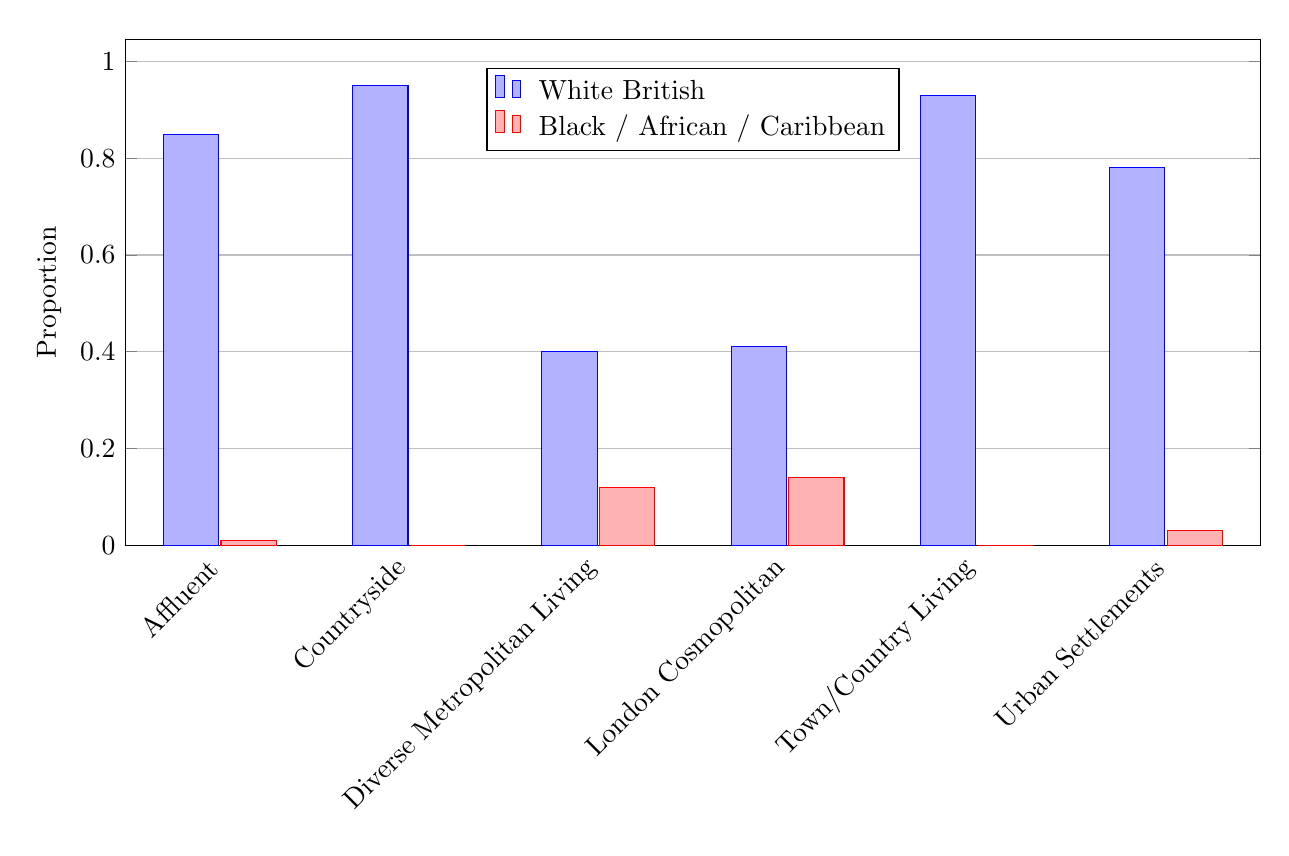
\begin{tikzpicture}
\begin{axis}[
    width  = 16cm,
    height = 8cm,
    major x tick style = transparent,
    ybar=2*\pgflinewidth,
    bar width=20pt,
    ymajorgrids = true,
    ylabel={Proportion},
	symbolic x coords={Affluent, Countryside, Diverse Metropolitan Living, London Cosmopolitan, Town/Country Living, Urban Settlements},
    xtick = data,
    scaled y ticks = false,
    enlarge x limits=0.10,
    x tick label style={anchor=east,rotate=45},  
    ymin=0,
    legend cell align=left,
    legend style={
            at={(0.5,0.78)},
            anchor=south,
            column sep=1ex
    }
]
    \addplot
        coordinates {(Affluent,0.85) (Countryside,0.95) (Diverse Metropolitan Living,0.4) (London Cosmopolitan,0.41) (Town/Country Living,0.93) (Urban Settlements,0.78)};

    \addplot
         coordinates {(Affluent,0.01) (Countryside,0) (Diverse Metropolitan Living,0.12) (London Cosmopolitan,0.14) (Town/Country Living,0) (Urban Settlements,0.03)};
    \legend{White British,Black  / African / Caribbean}
\end{axis}
\end{tikzpicture}
\end{document}